\chapter{非编码 RNA 与转录后调控}\label{ch:b3:rna-regulation}

1990 年，两位植物生物学家想让矮牵牛花变得更深的紫色，
为此给它们额外导入了一份色素合成酶基因的拷贝。近一半转基因植株
开出的花是白色的，或是紫色中夹着白色斑块：
外源基因不仅使自身沉默，也使植株自身的那份拷贝沉默。
八年后，两位线虫遗传学家向
\emph{Caenorhabditis elegans} 体内注射 RNA，发现与某一肌肉基因序列匹配的双链 RNA
能使该基因沉默，无论在被注射的线虫体内还是在其后代中，
效力远胜于任一单链。这两个谜题
有着同一个答案：细胞中存在一套机制，能利用短链 RNA 寻找并沉默序列互补的 RNA。
这套机制，以及信使 RNA 在转录之后经历的更广泛的调控，
包括如何剪接、被送往何处、寿命多长以及是否被翻译，
正是本章的主题。本科一年级分册把基因视为
在启动子处开或关的单位；
本章则让转录本本身
成为调控的对象。

\section{细胞中的 RNA 普查}

\begin{definition}[非编码 RNA]\label{def:b3:rna-regulation:ncrna}
\index{非编码 RNA}\index{微 RNA}\index{小干扰 RNA}\index{Piwi 互作 RNA}\index{长链非编码 RNA}\index{核小 RNA}
称\emph{非编码 RNA}（ncRNA）为以 RNA 自身发挥功能的转录本，
而非充当蛋白质模板。除翻译所用的核糖体 RNA 与转运 RNA 外，
以及剪接体的\emph{核小 RNA}（snRNA），真核细胞还含有：
\emph{微 RNA}
（miRNA），\numrange{21}{23}~个核苷酸，由细胞自身转录本中的发夹结构切割而成，
引导对部分互补的信使 RNA 进行抑制；
\emph{小干扰 RNA}（siRNA），长度相同，
由长双链 RNA 切割而来，引导对完全配对的靶标进行切割；
\emph{Piwi 互作 RNA}（piRNA），
\numrange{26}{31}~个核苷酸，在生殖系中针对
转座子发挥作用；小核仁 RNA 引导 rRNA 的修饰；
以及\emph{长链非编码 RNA}（lncRNA），即长度超过
\qty{200}{nt}、且无有意义开放阅读框的转录本，其中
\emph{\omterm{def:b3:chromatin-epigenetics:x-inactivation}{Xist}}（见\cref{ch:b3:chromatin-epigenetics}）是
研究得最透彻的一种。编码蛋白质的外显子约占人类基因组的 \qty{1.5}{\%}，
其余序列中有很大一部分在某些细胞的某些时刻会被转录，
但这些转录中有多少具有功能，
仍是一个悬而未决的问题。
\end{definition}

\begin{remark}[丰度不等于功能]\label{rem:b3:rna-regulation:function}
一个转录本被检测到，可能只是因为聚合酶有“渗漏”，而并非因为 RNA 确实发挥了作用；
大多数 \omterm{def:b3:rna-regulation:ncrna}{lncRNA} 每个细胞中的拷贝数少于 1 个，保守性差，缺失后也可有可无。
检验功能的标准是遗传学的：移除的是 RNA 本身而非仅其 DNA，
并由此出现表型。
\emph{\omterm{def:b3:chromatin-epigenetics:x-inactivation}{Xist}}、微 RNA 与 \omterm{def:b3:rna-regulation:ncrna}{piRNA} 均明确通过了这一检验；
在数以万计已注释的 \omterm{def:b3:rna-regulation:ncrna}{lncRNA} 中，
迄今只有数百个通过了检验。
\end{remark}

\section{RNA 干扰与微 RNA}

\begin{definition}[RNA 干扰]\label{def:b3:rna-regulation:rnai}
\index{RNA 干扰}\index{Dicer}\index{Argonaute}\index{RISC}
\emph{RNA 干扰}（RNAi）是指对某一基因的序列特异性沉默，
由双链 RNA 衍生的小 RNA 介导。酶
\emph{Dicer}（一种 RNase III）能将长双链 RNA
切割为 \numrange{21}{23}~个核苷酸的双链体，3$'$ 端带有两个核苷酸的
突出末端；每个双链体中的一条链，即引导链，被装入一种
\emph{Argonaute} 蛋白，形成 \emph{RNA 诱导沉默
复合体}（RISC）。引导链与互补的靶 RNA 配对，
Argonaute 的核酸内切酶结构域，在与引导链第 10
和第 11 位核苷酸相对的位置切割靶标；切割后的 RNA 被降解，
RISC 随即释放，去寻找下一个靶标。在植物、线虫和真菌中，
依赖 RNA 的 RNA 聚合酶以靶 RNA 为模板合成新的双链 RNA，
使信号得以放大并扩散；哺乳动物缺少这一步骤。
\end{definition}

\begin{proof}[证据]
纳波利、勒米厄和约根森（1990）向矮牵牛中额外导入一个查耳酮
合酶基因，以加深花色；其中 \qty{42}{\%}
的转化体开出白花或杂色花，转基因与内源基因同时被沉默，
即“共抑制”。郭和肯普斯（1995）发现，
针对 \emph{C.~elegans} 某一基因的反义 RNA 能使该基因沉默，
但有义对照同样如此。法尔、梅洛等人（1998）
解决了这一悖论：他们制备的单链 RNA 中混有双链，纯化后的
双链 RNA 针对 \emph{unc-22}，注入线虫后，在每个细胞仅几个分子的浓度下
即可引发抽动性的 \emph{unc-22} 表型，
而纯有义或纯反义 RNA 几乎没有效果；沉默效应
扩散到远离注射部位的组织，并
传递至后代。哈密顿与鲍尔科姆（1999）检测到沉默植株中的
\qty{25}{nt} 的 RNA，扎莫尔等人（2000）
在果蝇提取物中证明，双链 RNA 被切割成这类小片段，
而靶标则以
\qty{21}{nt} 为间隔被切断。
\end{proof}

\begin{omfigure}
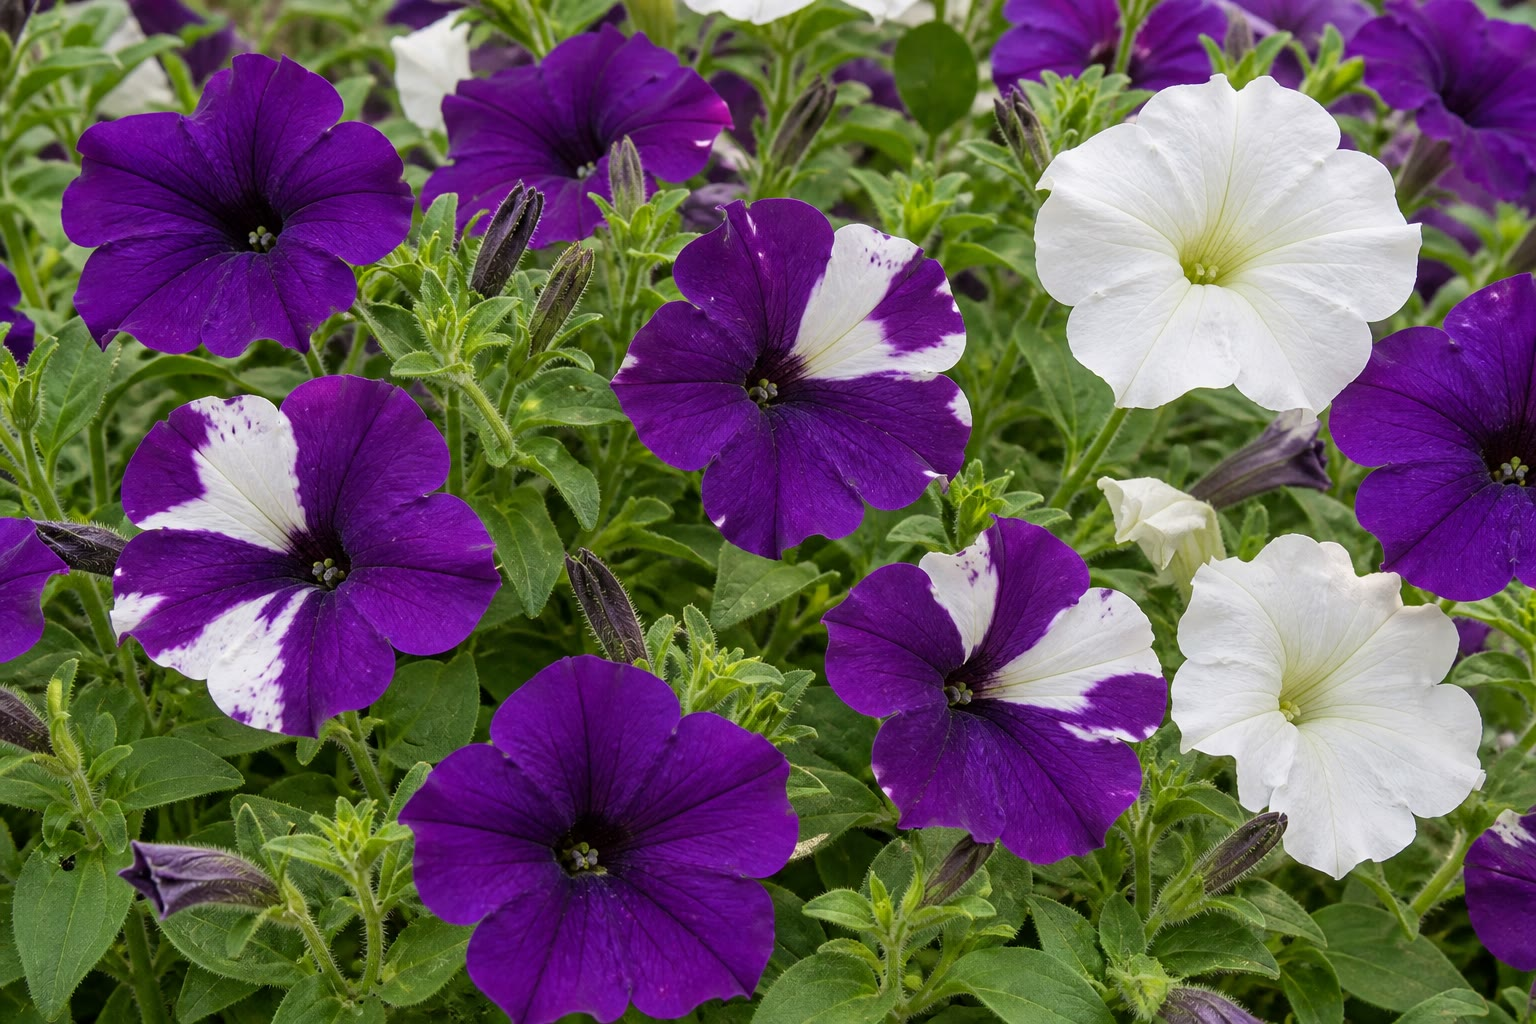
\includegraphics[width=0.46\linewidth]{images/book5/ai/b5-02-petunia-cosuppression.jpg}\hspace{0.04\linewidth}
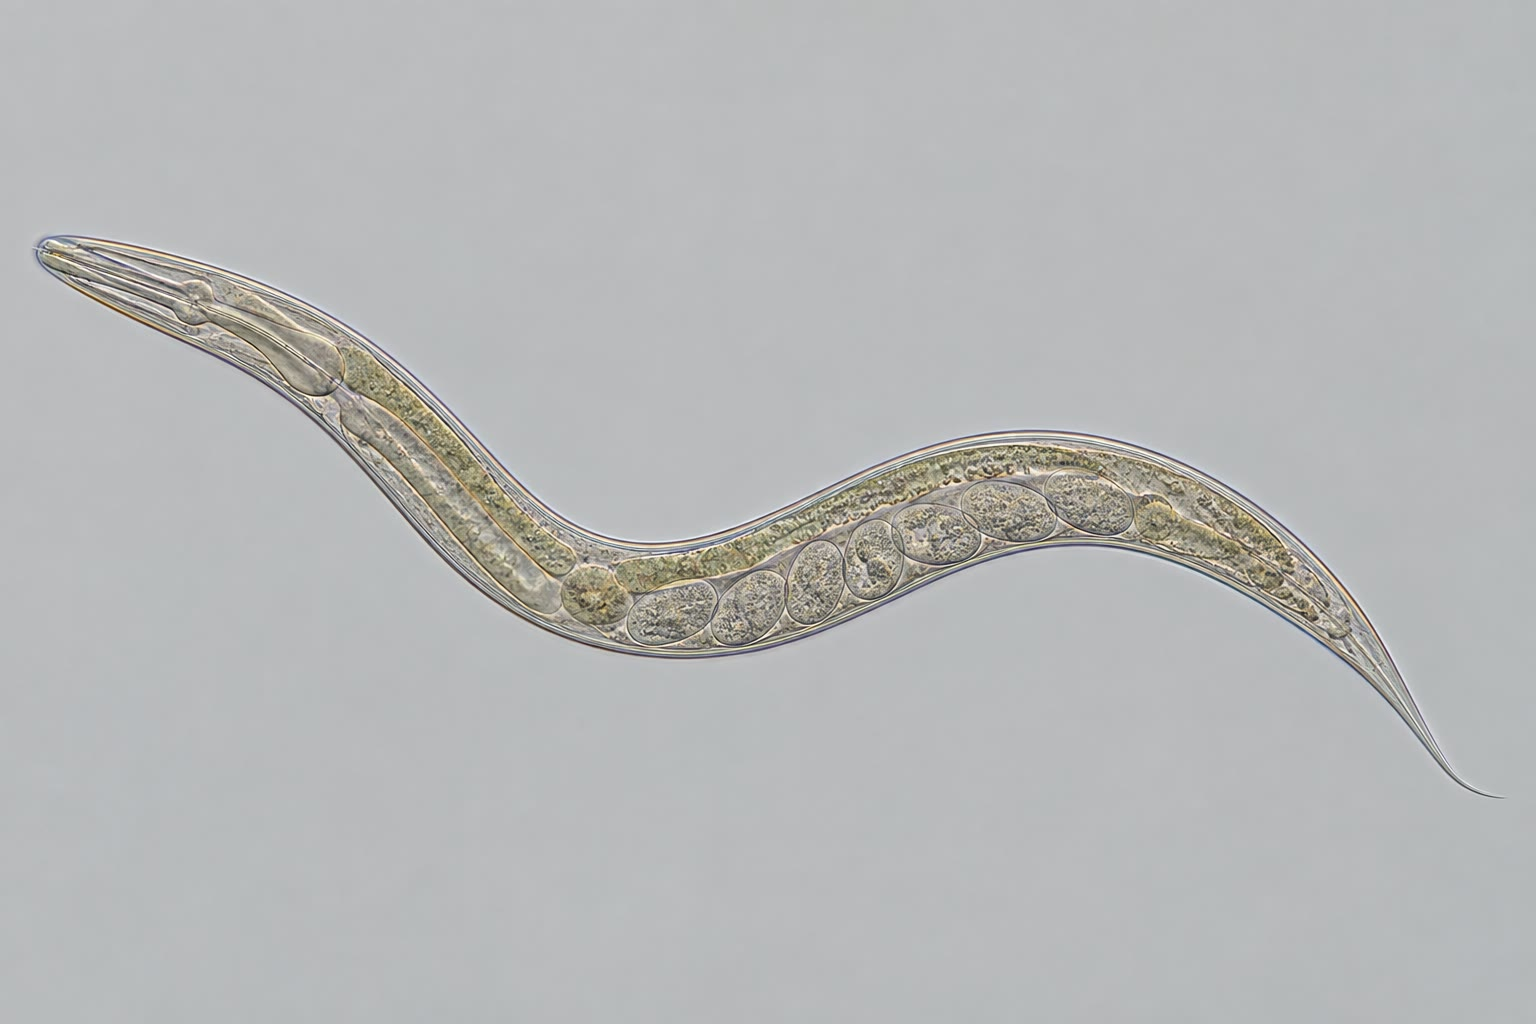
\includegraphics[width=0.46\linewidth]{images/book5/ai/b5-02-c-elegans.jpg}

{\small 左：携带额外色素基因、带有共抑制白色斑块的矮牵牛花。右：线虫
\emph{Caenorhabditis
elegans}，体长约 1 毫米、体态透明，在其体内注射的
双链 RNA 使整个个体中与之匹配的基因沉默，并
使其后代同样沉默。}
\end{omfigure}

\begin{definition}[微 RNA]\label{def:b3:rna-regulation:mirna}
\index{微 RNA!生物合成}\index{Drosha}\index{种子序列}
\emph{微 RNA}是由基因组编码的，既可位于其自身基因中，也可位于
蛋白质编码基因的内含子中，由 RNA 聚合酶 II 转录为较长的初级转录本
（pri-miRNA），其中含有一个约
\qty{70}{nt} 的发夹结构。在细胞核中，RNase III \emph{Drosha} 与其
伴侣 DGCR8 一起将发夹切下（即前体 \omterm{def:b3:rna-regulation:ncrna}{miRNA}，pre-miRNA）；exportin-5 将其
运至细胞质，在那里 \omterm{def:b3:rna-regulation:rnai}{Dicer} 去除环结构，留下
一个 \qty{22}{nt} 的双链体。其中一条链被装入 \omterm{def:b3:rna-regulation:rnai}{Argonaute}。成熟的微 RNA
主要通过其\emph{种子序列}识别靶标，
即第 2 至 8 位核苷酸，通常与信使 RNA 的 3$'$ 非翻译区中的位点配对；
其余部分的配对并不完全，因此靶标并不被切割，
而是被抑制：\omterm{def:b3:rna-regulation:rnai}{RISC} 招募能够缩短
poly(A) 尾、去除帽子结构并抑制翻译的蛋白质，使信使 RNA 的
降解也因此加快。由于种子序列只有 7 个核苷酸，一个微 RNA
可有数百个靶标；超过一半的人类蛋白质编码基因
携带保守位点，这些位点可与数百种
可靠鉴定的人类微 RNA 中至少一种相结合。
\end{definition}

\begin{proof}[证据]
\emph{lin-4}，一个使线虫由第一
幼虫期进入第二期所必需的基因，由李、芬鲍姆和安布罗斯（1993）发现，
编码的不是蛋白质，而是一条 \qty{22}{nt} 的 RNA，与七个
位点互补，位于 \emph{lin-14} 信使 RNA 的 3$'$ 非翻译区中，
即已知受其抑制的基因。幼虫进入第二阶段时，
LIN-14 蛋白消失，而其 mRNA 仍然存在：抑制是
转录后的。莱因哈特等人（2000）又发现了另一条这样的
RNA \emph{let-7}，控制幼虫后期的阶段转换；帕斯奎内利
（2000）在果蝇和人类中也发现了 \emph{let-7}，序列相同，
这使线虫中的一个奇特现象成为普遍机制。
\end{proof}

\begin{omfigure}
\begin{tikzpicture}[every node/.style={font=\scriptsize}, >=stealth]
  % nucleus box
  \draw[rounded corners=8pt, thick, gray!60, fill=gray!6] (-0.4,-1.1) rectangle (5.2,2.7);
  \node[gray, anchor=south west] at (-0.3,-1.05) {细胞核};
  % gene and pri-miRNA
  \draw[very thick, omDef] (0,2.0) -- (2.4,2.0); \node[above] at (1.2,2.05) {miRNA 基因，Pol II};
  \draw[->, thick] (1.2,1.85) -- (1.2,1.35);
  % hairpin
  \draw[thick, omThm!70!black] (0.2,1.0) -- (0.9,1.0) .. controls (1.0,1.0) and (1.05,0.9) .. (1.1,0.5) .. controls (1.15,0.1) and (1.25,0.1) .. (1.3,0.5) .. controls (1.35,0.9) and (1.4,1.0) .. (1.5,1.0) -- (2.2,1.0);
  \draw[thick, omThm!70!black] (1.1,0.5) -- (1.3,0.5);
  \node[below] at (1.2,0.0) {pri-miRNA 发夹};
  % Drosha
  \draw[thick, fill=omExo!35] (2.9,0.7) ellipse (0.55 and 0.28); \node at (2.9,0.7) {Drosha};
  \draw[->, thick] (2.3,0.85) -- (2.4,0.75);
  \draw[->, thick] (3.5,0.7) -- (4.2,0.7) node[midway, above] {切割};
  % pre-miRNA
  \draw[thick, omThm!70!black] (4.3,0.9) .. controls (4.5,0.9) and (4.55,0.4) .. (4.6,0.1) .. controls (4.65,-0.2) and (4.75,-0.2) .. (4.8,0.1) .. controls (4.85,0.4) and (4.9,0.9) .. (5.1,0.9);
  \node[below, align=center] at (4.7,-0.25) {前体 miRNA\\\qty{70}{nt}};
  % export
  \draw[->, thick] (5.35,0.4) -- (6.3,0.4) node[midway, above, xshift=0.2cm] {exportin-5 输出};
  % cytoplasm
  \node[gray, anchor=north west] at (5.5,2.65) {细胞质};
  \draw[thick, fill=omExo!35] (6.9,0.4) ellipse (0.5 and 0.28); \node at (6.9,0.4) {Dicer};
  \draw[->, thick] (7.45,0.4) -- (8.1,0.4);
  \draw[thick, omThm!70!black] (8.2,0.55) -- (9.6,0.55); \draw[thick, omThm!70!black] (8.35,0.25) -- (9.75,0.25);
  \node[below, align=center] at (8.95,0.15) {\qty{22}{nt} 双链体};
  \draw[->, thick] (8.95,-0.4) -- (8.95,-0.9) node[midway, right] {一条链被装入};
  % RISC on mRNA
  \draw[thick, fill=omProp!35] (8.95,-1.45) ellipse (0.85 and 0.35); \node at (8.95,-1.45) {Argonaute};
  \draw[thick, omThm!70!black] (8.3,-1.85) -- (9.6,-1.85);
  \draw[very thick, omDef] (5.6,-2.15) -- (11.4,-2.15);
  \node[below] at (6.4,-2.2) {mRNA：编码区}; \node[below] at (10.3,-2.2) {3$'$ UTR，靶位点};
  \draw[omDef, thick] (11.4,-2.15) -- (11.8,-2.15) node[right] {AAAA};
  \draw[->, thick, omThm] (9.9,-1.5) -- (10.9,-1.5) node[right, align=left] {去腺苷酸化，\\降解，\\翻译减少};
  \node[below, align=center] at (8.95,-2.7) {种子序列（nt 2--8）\\与靶位点配对};
\end{tikzpicture}

{\small 微 RNA 的生成。发夹结构从初级
转录本上被细胞核中的 \omterm{def:b3:rna-regulation:mirna}{Drosha} 酶切下，输出后被 \omterm{def:b3:rna-regulation:rnai}{Dicer} 酶修剪为一个
\qty{22}{nt} 双链体，一条链装入 \omterm{def:b3:rna-regulation:rnai}{Argonaute} 蛋白。\omterm{def:b3:rna-regulation:mirna}{种子
序列}与信使 RNA 的 3$'$ UTR 中的位点配对，信使
RNA 被去腺苷酸化、降解，翻译减少。}
\end{omfigure}

\begin{theorem}[微 RNA 对信使 RNA 水平和速度的影响]\label{thm:b3:rna-regulation:mirna-kinetics}
\index{mRNA 半衰期}\index{响应时间}
信使 RNA 以恒定速率 $k$ 合成，并以
一级速率 $\gamma$ 降解；水平为 $R$ 的微 RNA 增加一项衰减
$\gamma' R\, m$，则 mRNA 水平 $m(t)$ 服从
\[
\frac{\mathrm{d}m}{\mathrm{d}t} = k - (\gamma + \gamma' R)\, m,
\qquad
m^{*} = \frac{k}{\gamma + \gamma' R},
\qquad
m(t) = m^{*} + (m_{0} - m^{*})\,e^{-(\gamma + \gamma' R)t}.
\]
微 RNA 使稳态值降低 $1 + \gamma' R/
\gamma$ 倍，并使 $m$ 的任一变化的时间常数由
$1/\gamma$ 变为 $1/(\gamma + \gamma' R)$，缩短倍数相同。
受微 RNA 调控的基因因此既更平稳又更快：它
启动子改变后，它更快达到新的稳态，并且
其转录中的波动得到阻尼。
\end{theorem}
\begin{proof}
该方程为常系数线性方程，其不动点为
$m^{*}$，即右端为零处；令 $u = m - m^{*}$，
得 $\mathrm{d}u/\mathrm{d}t = -(\gamma + \gamma' R)\,u$，由此
得指数形式。趋近的半时为 $\ln 2/(\gamma + \gamma'
R)$，又 $\gamma = \ln 2 / t_{1/2}$，其中 $t_{1/2}$ 为信使
RNA 的自然半衰期。
\end{proof}

\begin{example}[四倍抑制]\label{ex:b3:rna-regulation:fourfold}
一条自然半衰期为 \qty{30}{min} 的信使 RNA（$\gamma =
\qty{0.023}{min^{-1}}$），以 $k = 2$ 个分子每分钟的速率转录，
稳定在 $m^{*} = 2/0.023 \approx 87$ 个拷贝每细胞，并
启动子改变后，需 \qty{30}{min} 才能移动到
新水平的一半。一个使衰减速率增为三倍的微 RNA（$\gamma' R = 3\gamma$）
可使其降至 $22$ 个拷贝，并将半时缩短为 \qty{7.5}{min}。
同一组数字倒过来看，说明了为何微 RNA 敲除常表现为轻微的
表型：一条本身受到缓冲的信使 RNA 出现四倍变化，
下游的缓冲作用可使生物体基本保持正常，此效应
只在压力下或时序上显现。
\end{example}

\begin{omfigure}
\begin{tikzpicture}
\begin{axis}[
  width=0.7\linewidth, height=5.6cm,
  axis x line=bottom, axis y line=left,
  xmin=0, xmax=120, ymin=0, ymax=100,
  xlabel={启动子开启后的时间（分钟）}, ylabel={每细胞 mRNA 数},
  xlabel style={font=\small, at={(axis description cs:0.5,-0.12)}, anchor=north},
  ylabel style={font=\small},
  tick label style={font=\small}, xtick={0,30,60,90,120}, ytick={0,22,50,87},
  clip=false,
]
\addplot[very thick, omDef, domain=0:120, samples=80] {87*(1-exp(-0.0231*x))};
\addplot[very thick, omThm, domain=0:120, samples=80] {21.7*(1-exp(-0.0924*x))};
\addplot[dashed, gray, domain=0:120, samples=2] {87};
\addplot[dashed, gray, domain=0:120, samples=2] {21.7};
\node[font=\scriptsize, omDef, anchor=south west] at (axis cs:5,90) {无微 RNA：$m^{*} = 87$，半时 \qty{30}{min}};
\node[font=\scriptsize, omThm, anchor=south west] at (axis cs:40,24) {有微 RNA，$\gamma' R = 3\gamma$：$m^{*} = 22$，半时 \qty{7.5}{min}};
\end{axis}
\end{tikzpicture}

{\small 启动子开启后信使 RNA 的积累过程，
数字取自\cref{ex:b3:rna-regulation:fourfold}。
微 RNA 使平台值降为原来的四分之一，且达到平台的时间缩短为四分之一。}
\end{omfigure}

\begin{method}[用 RNAi 敲低基因]\label{met:b3:rna-regulation:knockdown}
\index{敲低}\index{shRNA}
若要在不改动 DNA 的前提下沉默某个基因：
(1) 选取该基因信使 RNA 上独有的 \qty{21}{nt} 序列，
并避免与其他基因发生\omterm{def:b3:rna-regulation:mirna}{种子序列}匹配；
(2) 以合成 \omterm{def:b3:rna-regulation:ncrna}{siRNA} 双链体的形式导入（作用是暂时的，
约持续数天），或以短发夹 RNA（\omterm{met:b3:rna-regulation:knockdown}{shRNA}）的形式由载体表达导入，
\omterm{def:b3:rna-regulation:rnai}{Dicer} 对其持续加工；在线虫中，
则让动物取食表达双链 RNA 的细菌；(3) 用定量 PCR 测量信使 RNA，
用免疫印迹测量蛋白质，
预期下降 \qtyrange{70}{95}{\%}，而非像敲除那样完全消失；
(4) 用第二条不重叠的 \omterm{def:b3:rna-regulation:ncrna}{siRNA} 和 RNAi 抗性版本的基因进行拯救实验，
以排除脱靶效应。
\omterm{met:b3:rna-regulation:knockdown}{敲低}是功能的部分、可逆的丧失；目前已获批准的、基于这一原理的基因疗法，
是针对肝脏信使 RNA（转甲状腺素蛋白、
PCSK9）递送 \omterm{def:b3:rna-regulation:ncrna}{siRNA}，并与肝细胞可摄取的糖类相连。
\end{method}

\section{守护基因组的小 RNA}

\begin{definition}[piRNA 与转座子沉默]\label{def:b3:rna-regulation:pirna}
\index{piRNA!乒乓循环}\index{转座子沉默}\index{杂种不育}
\emph{\omterm{def:b3:rna-regulation:ncrna}{piRNA}} 是长 \numrange{26}{31}~个核苷酸的 RNA，
不依赖 \omterm{def:b3:rna-regulation:rnai}{Dicer}，
由基因组中长的单链转录本加工而成，
这些转录本来自 \emph{\omterm{def:b3:rna-regulation:ncrna}{piRNA} 簇}——缺陷转座子拷贝的“墓地”
——并装载到生殖系中 \omterm{def:b3:rna-regulation:rnai}{Argonaute} 蛋白的 PIWI 亚家族中。
与转座子反义的 \omterm{def:b3:rna-regulation:ncrna}{piRNA} 引导对转座子转录本的切割；
被切下的片段成为新的正义 \omterm{def:b3:rna-regulation:ncrna}{piRNA}，它又切割簇转录本，
产生更多反义 \omterm{def:b3:rna-regulation:ncrna}{piRNA}——这就是\emph{乒乓}循环，
一种针对当前活跃转座子的扩增机制。
核 PIWI 蛋白还引导 H3K9 甲基化和 DNA 甲基化作用于转座子的基因组拷贝，
从而把 RNA 与\cref{ch:b3:chromatin-epigenetics}中的\omterm{def:b3:chromatin-epigenetics:nucleosome}{染色质}标记联系起来。
母体将其 \omterm{def:b3:rna-regulation:ncrna}{piRNA} 沉积于卵中；
一只其谱系从未接触过某种转座子的雌性，
对该转座子没有对应的 \omterm{def:b3:rna-regulation:ncrna}{piRNA}，
而她与携带该转座子的雄性所生的后代则不育——这就是\emph{杂种不育}，
最早见于实验室品系与野生品系之间的\emph{果蝇}杂交中。
\end{definition}

\begin{proposition}[RNA 导向的染色质沉默]\label{prop:b3:rna-regulation:rddm}
\index{RNA 导向的 DNA 甲基化}
在植物中存在一条专门的途径：RNA 聚合酶 IV 转录某一基因座，
RNA 依赖的 RNA 聚合酶将其合成为双链，
\omterm{def:b3:rna-regulation:rnai}{Dicer} 切割出 \qty{24}{nt} 的 \omterm{def:b3:rna-regulation:ncrna}{siRNA}，
\omterm{def:b3:rna-regulation:rnai}{Argonaute}~4 将其带回到同一基因座上 RNA 聚合酶 V 产生的新生转录本上，
并招募甲基转移酶 DRM2，
使转座子和重复序列的 DNA 发生甲基化；
这正是\omterm{prop:b3:chromatin-epigenetics:examples}{副突变}的机制。在裂殖酵母中，
来自着丝粒重复序列的 \omterm{def:b3:rna-regulation:ncrna}{siRNA} 招募 H3K9 甲基转移酶，
构建着丝粒所需的\omterm{def:b3:chromatin-epigenetics:nucleosome}{异染色质}。两种情况下，
RNA 都通过互补性在基因组中找到位置，并在那里写下\omterm{def:b3:chromatin-epigenetics:nucleosome}{染色质}标记：
这种标记具有序列特异性、能够自我强化，并可通过细胞分裂遗传下去。
\end{proposition}

\section{信使 RNA 的一生}

\begin{definition}[调控性剪接]\label{def:b3:rna-regulation:splicing}
\index{可变剪接!调控}\index{SR 蛋白}\index{hnRNP}\index{外显子跳跃}
可变剪接通过\emph{外显子跳跃}、
在互斥外显子之间进行选择、保留内含子，或使用可变的 5$'$ 或3$'$ 剪接位点，
由同一基因产生不同的信使 RNA。
它受 RNA 结合蛋白调控，
这些蛋白结合在剪接位点附近外显子和内含子中的序列元件上：
结合于外显子增强子的\emph{SR 蛋白}招募剪接体，
促进外显子被保留；结合于沉默子的\emph{hnRNP}蛋白则阻止这一过程，
而在某一特定细胞中，
结果取决于这两类蛋白的相对含量。
人类多外显子基因中超过\qty{90}{\%} 发生可变剪接；
\emph{Dscam} 基因在\emph{果蝇}中含有四个互斥外显子区块（分别有 12、
48、33 和 2 个可选外显子），
能够产生 \num{38016} 种不同的蛋白质，
每个神经元表达其中不同的一组，使其分支能够相互识别并避开。
\end{definition}

\begin{proof}[证据]
果蝇的性别由一条剪接级联决定。在雌性中，
\emph{Sex-lethal}（\emph{Sxl}）基因产生有功能的蛋白质；
SXL 是一种 RNA 结合蛋白，
它阻断自身转录本上的一个剪接位点（使带有终止密码子的外显子被跳过，
从而蛋白质得以持续产生），并阻断 \emph{transformer}转录本上的剪接位点，
迫使其走雌性剪接途径；
随后 TRA 与 TRA-2 结合在 \emph{doublesex} 转录本的外显子增强子上，
并引导产生雌性形式的 DSX 转录因子。
在雄性中，没有 SXL，上述转录本都走默认剪接，
\emph{transformer} 含有终止密码子，
DSX 则以雄性形式产生。果蝇所有的性二态特征都取决于产生的是哪种 DSX；
\emph{tra} 发生突变的雌性则发育为雄性。
\end{proof}

\begin{definition}[mRNA 稳定性与定位]\label{def:b3:rna-regulation:stability}
\index{AU 富含元件}\index{mRNA 定位}\index{铁应答元件}
信使 RNA 的\emph{半衰期}从数分钟到数天不等，
由其 3$'$ 非翻译区中的元件决定。
\emph{富含 AU 元件}（AUUUA 重复序列）存在于细胞因子、
生长因子和原癌基因的信使 RNA 中，结合这些元件的蛋白质招募去腺苷酸化酶，
使半衰期缩短至 \qtyrange{10}{30}{min}，
因此转录的一次爆发只会产生一次蛋白质爆发，之后不再增多；
去除这些元件的突变会导致过量表达，对某些原癌基因而言还会引发癌症。
\emph{定位元件}往往具有结构，它们被衔接蛋白结合，
把信使 RNA 连接到马达蛋白上：
\emph{bicoid} 和 \emph{oskar} 的信使 RNA 由动力蛋白和驱动蛋白沿微管运送到果蝇卵的两极，
$\beta$-肌动蛋白的信使 RNA 被运送到成纤维细胞的前沿，
而突触蛋白的信使 RNA 则被运入树突，
在那里按需翻译。
\emph{铁应答元件}（IRE）是一个茎环结构，
在铁缺乏时被铁调节蛋白 IRP1 和 IRP2 结合，它在两个不同位置发挥两种相反的作用：
在铁蛋白信使 RNA 的 5$'$ 非翻译区，
结合的 IRP 阻断核糖体；在转铁蛋白受体信使 RNA 的 3$'$ 非翻译区，
结合的 IRP 则保护转录本免受核酸酶降解。
\end{definition}

\begin{example}[铁，由一个发夹读取]\label{ex:b3:rna-regulation:iron}
铁含量低时，IRP 同时结合两种信使：铁蛋白（储存蛋白）不被翻译，
而摄取铁的转铁蛋白受体则变得稳定且丰富，
细胞因此储存更少、摄取更多。
铁含量高时，IRP1 转变为乌头酸酶（获得铁硫簇，并失去对 RNA 的亲和力），
IRP2 则被降解：铁蛋白得以翻译，受体信使在数分钟内衰减，
细胞因此储存更多、摄取更少。
无需改变转录。
铁蛋白 IRE 上的一个点突变若阻碍 IRP 结合，
会导致铁蛋白持续合成，
并引发遗传性高铁蛋白血症–白内障综合征。
\end{example}

\begin{omfigure}
\begin{tikzpicture}[every node/.style={font=\scriptsize}, >=stealth]
  \foreach \yy/\state in {2.2/低铁, -0.9/高铁} {
    \node[left, font=\small\bfseries] at (-0.2,\yy+0.35) {\state};
    % ferritin mRNA
    \draw[very thick, omDef] (0.3,\yy+0.6) -- (4.6,\yy+0.6); \node[below] at (3.3,\yy+0.4) {铁蛋白 mRNA};
    \draw[thick, omThm!70!black] (0.9,\yy+0.6) .. controls (0.9,\yy+1.15) and (1.3,\yy+1.15) .. (1.3,\yy+0.6); \node[below] at (1.1,\yy+0.55) {IRE};
    \draw[fill=omDef!20, thick] (2.2,\yy+0.42) rectangle (4.4,\yy+0.78);
    % TfR mRNA
    \draw[very thick, omDef] (6.2,\yy+0.6) -- (10.6,\yy+0.6); \node[below, font=\tiny] at (7.1,\yy+0.4) {转铁蛋白受体 mRNA};
    \draw[fill=omDef!20, thick] (6.4,\yy+0.42) rectangle (8.6,\yy+0.78);
    \foreach \x in {9.0,9.5,10.0} \draw[thick, omThm!70!black] (\x,\yy+0.6) .. controls (\x,\yy+1.1) and (\x+0.35,\yy+1.1) .. (\x+0.35,\yy+0.6);
    \node[below, font=\tiny] at (9.9,\yy+0.55) {3$'$ UTR 中的 IRE};
  }
  % low iron: IRP bound
  \draw[thick, fill=omProp!40] (1.1,3.35) ellipse (0.4 and 0.24); \node at (1.1,3.35) {IRP};
  \node[right, omThm] at (1.55,3.35) {核糖体受阻：无铁蛋白};
  \foreach \x in {9.18,9.68,10.18} { \draw[thick, fill=omProp!40] (\x,3.35) ellipse (0.28 and 0.2); }
  \node[above, omMeth!70!black] at (9.7,3.75) {免受核酸酶降解：受体稳定且丰富};
  \node[below, omMeth!70!black] at (1.1,1.75) {储存更少};
  \node[below, omMeth!70!black] at (7.4,1.75) {摄取更多};
  % high iron: IRP off
  \node[right, omMeth!70!black] at (1.55,0.25) {已翻译：合成铁蛋白};
  \node[right, omThm, align=left] at (10.7,-0.3) {核酸酶：\\mRNA 降解};
  \node[below, omThm] at (1.1,-1.35) {储存更多};
  \node[below, omThm] at (7.4,-1.35) {摄取更少};
\end{tikzpicture}

{\small \omterm{def:b3:rna-regulation:stability}{铁应答元件}。低铁时，铁调节蛋白
结合 IRE 发夹：在铁蛋白信使的 5$'$ 端，
它阻止翻译；在转铁蛋白受体信使的 3$'$ 端，
它阻止核酸酶。高铁时，该蛋白同时释放两者：
铁蛋白得以合成，受体信使降解。}
\end{omfigure}

\begin{proposition}[翻译控制]\label{prop:b3:rna-regulation:translation}
\index{翻译控制}\index{eIF2}\index{核糖开关}\index{上游开放阅读框}
起始步骤通常是\omterm{prop:b3:rna-regulation:translation}{翻译控制}的主要位点。
起始因子 \emph{\omterm{prop:b3:rna-regulation:translation}{eIF2}} 被激酶磷酸化。这些激酶可感知
氨基酸饥饿、未折叠蛋白、病毒双链 RNA 或血红素缺乏，
磷酸化后数分钟内即关闭一般的起始过程，只有少数具有特殊结构特征的信使例外，
尤其是带有\emph{\omterm{prop:b3:rna-regulation:translation}{上游开放阅读框}}的信使。\omterm{prop:b3:rna-regulation:translation}{上游开放阅读框}是位于 5$'$ 非翻译区的短阅读框，
通常会捕获核糖体；在应激条件下，这些核糖体被绕过，使应激反应因子
（酵母中的 GCN4，哺乳动物中的 ATF4）
得以合成，
恰在其他蛋白都不被合成时。
帽结合因子 eIF4E 受 4E 结合蛋白抑制而失活，
直至生长信号激酶 mTOR 使其磷酸化：
只有营养物质和生长因子发出信号时，细胞才以全速翻译。
在细菌中，\emph{\omterm{prop:b3:rna-regulation:translation}{核糖开关}}无需任何蛋白即可完成调控：
结构化的 5$'$ 区域结合一种代谢物（焦磷酸硫胺素、
S-腺苷甲硫氨酸或嘌呤），结合后发生重折叠，以掩埋核糖体结合位点，
或形成转录终止子，
从而使生物合成操纵子在其产物充足时关闭。
\end{proposition}

\begin{omfigure}
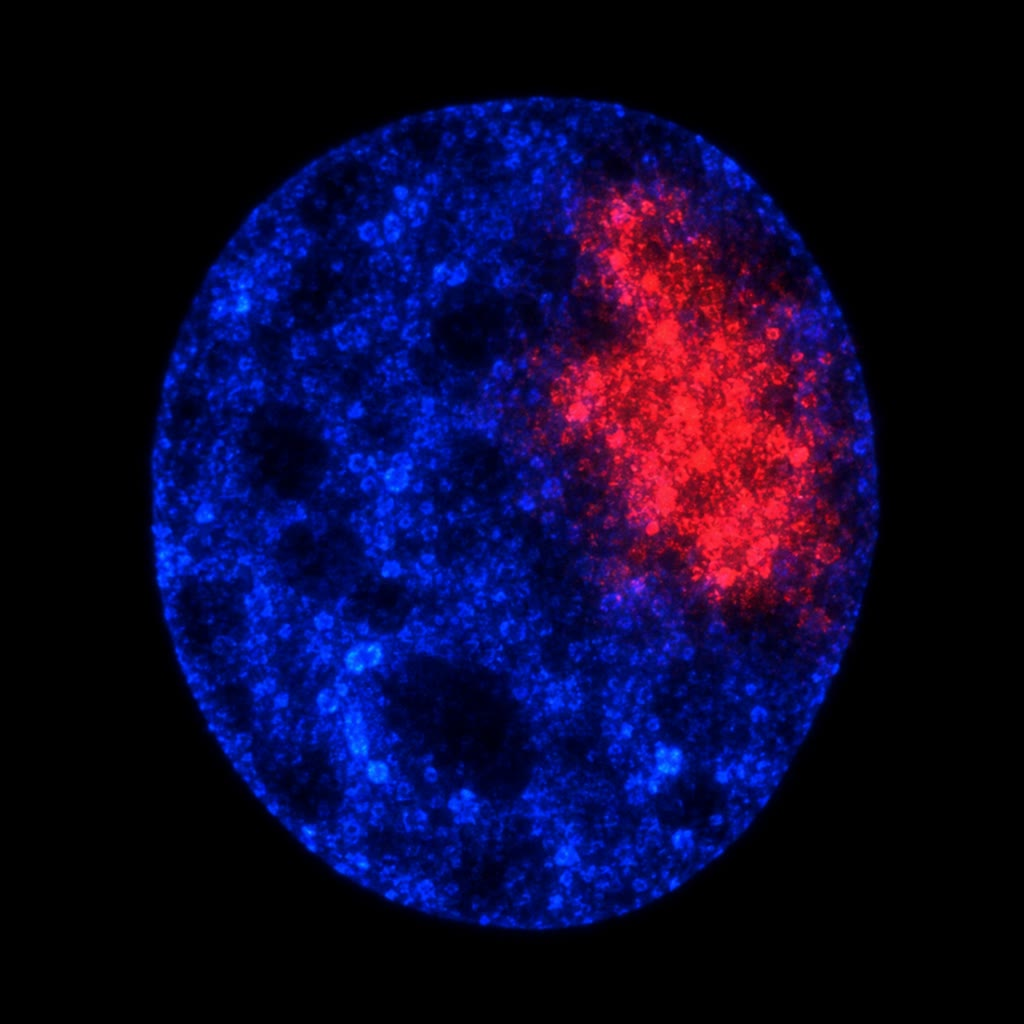
\includegraphics[width=0.36\linewidth]{images/book5/ai/b5-02-lncrna-nucleus.jpg}

{\small 长链非编码 RNA 的作用：\emph{\omterm{def:b3:chromatin-epigenetics:x-inactivation}{Xist}} 转录本
（红色），经荧光杂交检测，包覆雌性细胞核中
一条 X 染色体所占的区域（DNA 呈蓝色）。}
\end{omfigure}

\begin{remark}[转录后控制的意义]\label{rem:b3:rna-regulation:why}
转录控制通过细胞核发挥作用，新信使在被合成、输出并翻译之前，
通常会有数分钟至数小时的延迟。
对信使本身的控制作用于需要蛋白的地方，在数秒至数分钟内完成，
并可以是局部的：单个树突上的一个突触处
翻译某一信使，成纤维细胞的前沿处
合成肌动蛋白以便爬行。它还使一个基因产生多种蛋白，
并使一个信号——铁、氨基酸或微 RNA——能够同时协调
数百条信使，
而无需触及任何一个启动子。
\end{remark}

\section{练习}

\begin{exercise}[$\star$]\label{exo:b3:rna-regulation:1}
按来源、长度、对 \omterm{def:b3:rna-regulation:rnai}{Dicer} 的依赖性，
以及对靶标的作用，区分 \omterm{def:b3:rna-regulation:ncrna}{miRNA}、\omterm{def:b3:rna-regulation:ncrna}{siRNA} 和 \omterm{def:b3:rna-regulation:ncrna}{piRNA}。
\end{exercise}

\begin{exercise}[$\star$]\label{exo:b3:rna-regulation:2}
追踪一条微 RNA 从基因到被抑制信使的生物合成过程，
并指出每一步切割所用的酶。
\end{exercise}

\begin{exercise}[$\star$]\label{exo:b3:rna-regulation:3}
早期实验中，为何将 \emph{unc-22} 的有义 RNA 注入线虫后，
该基因会被沉默？Fire 和 Mello 改变了什么？
\end{exercise}

\begin{exercise}[$\star$]\label{exo:b3:rna-regulation:4}
细胞缺铁时，铁蛋白和转铁蛋白受体会发生什么变化？
在每种情况下，受控的是表达的
哪一步？
\end{exercise}

\begin{exercise}[$\star\star$]\label{exo:b3:rna-regulation:5}
一条信使 RNA 的半衰期为 \qty{2}{h}，以每分钟 $5$
个分子的速率合成。求其稳态水平，再求
微 RNA 使其降解速率加倍时的水平与半衰时间。
\end{exercise}

\begin{exercise}[$\star\star$]\label{exo:b3:rna-regulation:6}
一段七个核苷酸的\omterm{def:b3:rna-regulation:mirna}{种子序列}与随机序列匹配的概率为
$4^{-7}$。在一组 \num{20000} 条信使 RNA 中，其 3$'$ 非翻译区
平均为 \qty{1000}{nt}，则一个微 RNA 的\omterm{def:b3:rna-regulation:mirna}{种子序列}
偶然匹配多少个位点？那么，什么才能区分真正的靶标？
\end{exercise}

\begin{exercise}[$\star\star$]\label{exo:b3:rna-regulation:7}
预测下列果蝇的性别：(a) 具有 \emph{tra} 功能缺失突变
且含两条 X 染色体的果蝇；(b) 由组成型转基因表达
TRA，含一条 X 染色体的果蝇；(c) 完全缺失 \emph{dsx} 的果蝇。
\end{exercise}

\begin{exercise}[$\star\star$]\label{exo:b3:rna-regulation:8}
一条原癌基因信使 RNA 的半衰期通常为 \qty{15}{min}，
这归因于一个富含 AU 元件。一次染色体易位
删除了该元件，半衰期变为 \qty{3}{h}。若翻译与蛋白质降解均不变，
蛋白质水平将升高多少倍？
为何它会致癌，即使蛋白质本身是正常的？
\end{exercise}

\begin{exercise}[$\star\star$]\label{exo:b3:rna-regulation:9}
某实验室的 \emph{Drosophila} 品系缺少 P 元件；野生
品系则携带 P 元件。请预测下列杂交后代的可育性：
(a) 实验室品系雌性 $\times$ 野生雄性，(b) 野生雌性 $\times$
实验室雄性，并用 \omterm{def:b3:rna-regulation:ncrna}{piRNA} 解释这种不对称性。
\end{exercise}

\begin{exercise}[$\star\star\star$]\label{exo:b3:rna-regulation:10}
利用\cref{thm:b3:rna-regulation:mirna-kinetics}，论证由信使 RNA 产生的蛋白质，
在相对意义上波动更小，前提是该信使 RNA 受微 RNA 调控
且两种情形下信使 RNA 的平均水平相等。
（蛋白质对信使 RNA 在其自身寿命内取平均，而信使 RNA
更新得更快。）细胞为何要为一个微 RNA 付出代价，
并提高转录速率，以获得相同的平均水平？
\end{exercise}

\begin{exercise}[$\star\star\star$]\label{exo:b3:rna-regulation:11}
在线虫中，一种 RNA 依赖性 RNA 聚合酶以靶信使 RNA 为模板
合成次级 \omterm{def:b3:rna-regulation:ncrna}{siRNA}；哺乳动物中则没有此酶。请分别预测，
单次注射双链 RNA 引起的沉默能否持续
经历多次细胞分裂，以及是否扩散至其他组织，
并说明这对 \omterm{def:b3:rna-regulation:ncrna}{siRNA} 药物的医学后果。
\end{exercise}

\begin{exercise}[$\star\star\star$]\label{exo:b3:rna-regulation:12}
一个新注释的 \omterm{def:b3:rna-regulation:ncrna}{lncRNA} 在心脏中表达。请设计
能够区分以下情形的实验：(a) 具有功能的 RNA，(b) 有功能的
转录行为而其 RNA 无关紧要，以及 (c) 噪声，
并说明每种情形预测的结果。
\end{exercise}

\section{问题：线虫的计时器}

\begin{problem}[{周末问题——\emph{lin-4}/\emph{lin-14}
开关，线虫的计时由信使 RNA 动力学决定，注入的 RNA
在胚胎分裂中被稀释，并通过
扩增得以挽救；铁调节子定量分析，并统计剪接，
最后得出抑制倍数、开关的半衰时间，以及
未经扩增的信号所能存活的分裂次数}]
\label{pb:b3:rna-regulation:1}
数据：\emph{lin-14} 信使 RNA 的合成速率为每细胞每分钟 $k = 3$
个分子，半衰期为 \qty{40}{min}。LIN-14 蛋白质以
每条信使 RNA 每分钟 $\beta = 2$ 的速率合成，半衰期为
\qty{3}{h}。自第二幼虫期开始，\emph{lin-4}
RNA 积累，并为信使 RNA 增加一项降解项 $\gamma' R = 3\gamma$，
并通过阻断翻译起始使 $\beta$ 减半。线虫胚胎
从一个细胞发育至孵化时约 \num{550} 个细胞；成虫
有 \num{959} 个体细胞。

\medskip
\noindent\textbf{第一部分——信使 RNA。}
\begin{enumerate}
  \item 求 $\gamma$ 以及 \emph{lin-14} 信使 RNA 在
        \emph{lin-4} 出现前的稳态水平。
  \item 求蛋白质的降解速率，以及 LIN-14 蛋白质的稳态
        水平。
  \item \emph{lin-4} 出现后，求信使 RNA 的新水平
        以及信使 RNA 的新时间常数。
  \item 求蛋白质的新稳态水平，以及
        蛋白质上的总抑制倍数。
  \item \emph{lin-4} 出现后，信使 RNA 需要多长时间才
        达到新水平的一半？蛋白质呢——哪一步
        限制开关的速度？
  \item 原始实验发现蛋白质已经消失，而 mRNA
        仍可检测到。这与你的计算结果是否一致？
        信使 RNA 残留的比例为多少？
\end{enumerate}

\medskip
\noindent\textbf{第二部分——稀释与扩增。}
\begin{enumerate}[resume]
  \item 向线虫性腺注射 $10^{6}$ 个
        双链 RNA 分子，平均分配给 \num{250} 个
        卵。每个卵中有多少个分子？
  \item 若每次分裂时分子仅是简单地分配，
        则 \num{550} 个细胞的孵化幼虫，每个细胞含有多少个分子？
        再经过多少次分裂，平均值将降至
        每个细胞不足一个？
  \item 法尔与梅洛在整个动物及其后代中观察到沉默，
        每细胞仅几个分子。请解释 RNA 依赖性 RNA 聚合酶
        对这一解释增加了什么，以及为何该效应
        仍会在数代之后减弱。
  \item 在无此类聚合酶的哺乳动物细胞中，一次 \omterm{def:b3:rna-regulation:ncrna}{siRNA} 转染
        将 \num{5000} 个双链体导入一个每日分裂的细胞，
        \omterm{def:b3:rna-regulation:rnai}{RISC} 稳定，但会因分裂而被稀释。经过多少天后，
        其数量降至 \num{100} 以下，这大致是有效沉默
        所需的数量？
  \item 一种针对肝脏信使 RNA 的治疗性 \omterm{def:b3:rna-regulation:ncrna}{siRNA} 仅给药一次，
        可持续起效六个月。肝细胞很少分裂。请解释
        为何第 10 题中的机制不会限制它，
        以及什么才会限制它。
  \item 一段七个核苷酸的\omterm{def:b3:rna-regulation:mirna}{种子序列}平均每
        $4^{7}$ 个核苷酸随机匹配一次。线虫转录组约有
        \qty{20}{Mb} 的 3$'$ 非翻译序列。\emph{lin-4} 有多少个偶然的
        种子匹配？遗传学家是如何知道
        哪个靶标才是真正重要的？
\end{enumerate}

\medskip
\noindent\textbf{第三部分——铁调控子。}
\begin{enumerate}[resume]
  \item 在富铁细胞中，转铁蛋白受体信使 RNA 的半衰期
        为 \qty{10}{min}；结合 IRP 后为 \qty{50}{min}。
        在转录不变的情况下，当铁变得匮乏时，
        信使 RNA 的水平将升高到原来的多少倍？
  \item 铁蛋白信使 RNA 的水平不变，但结合 IRP 时，
        其翻译速率（每分钟每个信使 RNA 产生的蛋白质数）
        由 $1$ 降至 $0.05$。铁蛋白合成下降了多少倍？
  \item 综合两者：摄取容量与储存容量之比
        在富铁状态与缺铁状态之间，
        改变了多少倍？
  \item IRP1 蛋白是 RNA 结合蛋白还是乌头酸酶，
        取决于它是否结合铁硫簇。
        请解释为何这使它成为铁本身的感受器，
        而非激素的感受器。
  \item 某患者携带铁蛋白 IRE 突变，使 IRP 无法结合。
        请预测铁蛋白水平和血清铁水平，
        并说明为何眼晶状体会受到影响。
  \item 用一句话解释，为何同一个发夹结构在一个位置上可以激活，
        而在另一个位置上却起抑制作用。
  \item IRP2 不含铁硫簇；铁含量高时，它会被
        一种泛素连接酶降解，而该连接酶自身的稳定
        性需要铁和氧气。细胞为何可能保留两种
        化学性质如此不同的感受器？
\end{enumerate}

\medskip
\noindent\textbf{第四部分——计算异构体数目。}
\begin{enumerate}[resume]
  \item \emph{Dscam} 的外显子块分别有 12、48、33 和 2 种
        相互排斥的可选形式。共有多少种异构体？若每个神经元
        随机表达约 $50$ 种，则任意两个给定神经元
        至少共享一种异构体的概率为多少？（可用 $1 - (1 -
        50/N)^{50}$。）
  \item 为何神经元拥有其相邻神经元几乎肯定不具备的异构体，
        会对它有利？
  \item 某基因含 $n$ 个盒式外显子，各外显子独立地被保留
        或被跳过，可产生多少种信使 RNA？当 $n = 10$ 时
        有多少种？为何某一特定细胞类型中的实际数目
        通常远小于此数？
  \item 在果蝇中，为何一只拥有两条 X 染色体、
        但 \emph{Sxl} 为无效等位基因的雌性个体会死亡，而不是
        简单地发育为雄性？（可考虑 X 计数系统还控制
        什么：X 连锁基因的\omterm{def:b3:chromatin-epigenetics:x-inactivation}{剂量补偿}。）
  \item SXL 促进其自身转录本的有效剪接。请解释为何这使性别决定
        成为一种记忆，在仅存在于早期胚胎中的 X 计数信号
        消失之后仍然持续存在，
        并将其与自我维持的开关相联系，这类开关
        在\cref{ch:b3:chromatin-epigenetics}中已有论述。
  \item 请归纳这一计时器：LIN-14 蛋白上的抑制倍数
        （第~4~题）、信使开关的半衰期
        （第~5~题），以及未经放大的信号
        在降至每个细胞一个分子以下之前
        所能经历的分裂次数（第~8~题）。
\end{enumerate}
\end{problem}
